%-*-texinfo-*-
%This is part of the "UFO:Alien Invasion"-Reference Manuals Tex sources.
%Copyright (C) 2006 Eric Goller.
%See the file ufo-manual_EN.tex for copying conditions.

%---------------------------------------------------------------------------
%							Version history
%
%  date		/		changes																	/		comment						/ author
%	06.10.06	/	rev. 0.0.5 (alpha) released											/	complete aspell-check		/	Elbenfreund
%	07.10.06	/	added the overdue geoscape screenshot					/											/	Elbenfreund
%	08.10.06	/	added promotion and badges										/											/	Elbenfreund
%					/	+ size-optimized geoscape sceenshots added			/											/
%
%---------------------------------------------------------------------------


\section{Geospace}

\subsection{Worldmap - an overview} 
Welcome to Geoscape! As said before UFO:AI distincts between two major aspects of the game - macromanagement and tactical combat. To put it simple one could say: Combat is where you earn the bucks (besides honor of cause ... ), Geoscape is where you spend em.

Geoscape itself basically consist of two screens. The first one is the world map. This is where you get in right after starting a new campaign and it is used to get the bigger picture as well as coordinating combat missions and intercepting enemy UFOs. Second is the base overview, where you improve infrastructures and order important decisions about equipment, research and production. In the following we will take a closer look at both of them.

Taking the following screenshot we will have a look at what we might want to use the world map for.
Please take notice of the fact that it is divided into day and night zones which actually influence any combat mission you get into (the day/night boarderline changes its shape according to the seasons as the relation earth to sun changes).\\

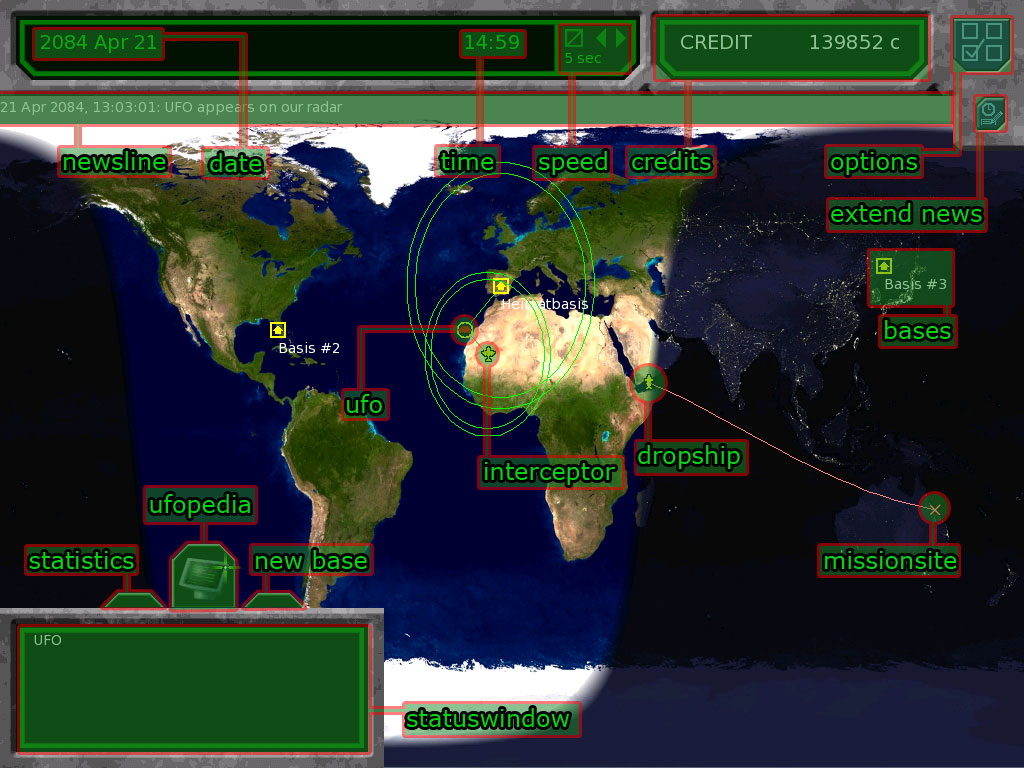
\includegraphics[width=\textwidth]{images/geoscape_final.jpg}

\newpage

\subsubsection{Statuswindow}
Here some general information(e.g. stats, descriptions) show up depending on the context. What is shown in detail will be explaint in the following.
\subsubsection{Statistics}
If you hover over those registers three different buttons will show up. While the very left one leads to some more detailed statistics about your attemp to save the world. Besides some more general information (like mission won/lost etc.) you can also find out about the attitude of all the UN countries paying you. Please be aware that if you fail to protect particular countries from alien invasions (maybe because your infrastructure are not well established in that region they will cut your rescources (financial and employees)
\subsubsection{Ufopedia}
Ufopedia is a comprehensive collection of usefull information about items, technologies, damage types and others. As your research proceeds Ufopedia grows as well, so make sure you check the latest news on your enemy's every now and then.
\subsubsection{New base}
Finally the right button gives you the chance to establish a new base anywhere (besides water) on the map. A new base, once you installed the required structures, gives additional radar-range, research and production capacities as well as new hangars for your aircrafts and is completely equal (also in administration) to your first base.
\subsubsection{Date}
Gives you the current date, so you know when its close to pay day. Please keep in mind that for mankind time is kind of running up. While you, in principle, have unlimited time at your hand, in fact aliens get stronger and better equipped as the game proceeds and you will have to catch up with them in order to beat them and save your beloved homeworld.
\subsubsection{Time}
Well, as you location isn't nailed down to one certain base this is just to illustrate how fast time proceeds. See also next paragraph.
\subsubsection{Gamespeed switch}
This is where you can adjust the gamespeed from 5secs (which is in fact pausing the game) over 5Min's up 1day steps. Whatever you put here, while you are in combat time is stoped and it will be all the same when you return from the field of honor.
\subsubsection{Credits}
Should be quite self-explaining. Never forget, you can't spend what you don't have.
\subsubsection{Options}
Gets you to the Options-menu where you can load and save your game as well as start a new one.
Through "exit" you reach the main menu where you can change game settings and continue your current game (via singleplayer $\rightarrow$ continue)
\subsubsection{news and extended news}
The permanent news line in the upper left always represents the latest news (such as promotions / cashflow / attacks / UFO-sightings) while the extended news button pops up a list of the last 20 newlines.
So whenever you notice news, make sure to check the button as well so you don't miss anything. 
\subsubsection{Bases}
Those yellow houses represent your bases. Circles around them (popping up later in the game) represent their radars range.  If you want to "enter" a base just click on its symbol.
\subsubsection{Your dropship}
This is the one that gets you squad to action. Clicking on it once brings up some general data about it (like fuel, speed, status and amount assigned soldiers) to the status screen. A second click while it's selected opens a submenu where you may give/change orders,e.g. sending it back home.
\subsubsection{Your interceptors}
Those fast ships job is to take enemy UFOs down. If it catches up with one the dogfight is going to be calculated based on both ships equipment and the result shown on screen. Just like one paragraph before a single click selects the interceptor (a further click to a certain spot on the map will order it to move it there) printing some general information in the status window. A second click while it is selected brings up a window where you might give more advanced orders to your ship.
\subsubsection{Upcomig missions}
This is where the action waits. Selecting a mission will give you a short description on the status screen while a second one makes you select a ship to bring in the troops you want.


\section{Your base}
Your bases have to furfil a wide range of tasks, ranging from researching and producing new equipment, gathering background information on the invaders and supplying the infrastructures to react on any alien attack via interceptors or dropships. You can change the name of your bases by clicking on the pen-icon right next to its name shown on base screen. Using the arrow icons you can also circle through all your current bases. In the following we will list all relevant screens so you can get familiar with the base management system step by step...

\subsection{Buildings}
This is where you order the construction of additional facilities for your base for example because you want to increase your research cap (lab) or fasten your soldiers healing process.
In fact all of this is irrelevant for your start-up base as hardly any research/production limit or medical care is implemented yet. Before you finally place a new building make sure you have read its according ufopedia entry. There you can find out if the new site requires additional buildings (for example a power plant) or what its concretee use is. Another important aspect when expanding your base is building time. Buildings vary quite strong in the amount of time needed to be finished once placed so it is important to consider this right from the start. Please also keep in mind that there are some quite elementary buildings needed in each base before the base is functional at all, in particular this is a power plant and command center. As said before, new bases can be build using the world-map so you don't need to place all facilities in one site as space is limited.

\subsection{Aircrafts}
This menu brings up a screen where you manage aircrafts in the according base. This includes not only equipping your vessels with your latest equipment but transferring them to another base or buying new ones. You can also circle through all your aircrafts using the left and right arrow icons in the window displaying the current aircraft. Even if it also possible to call an aircraft back to base or launch it using the buttons in this menu aircraft control is more likely to be done on the global map (as described before).
Propably the most important sub-menu here is "Equip Aircraft".  A click brings up a screen which allows you to choose which soldiers to assign to your selected aircraft. Obviously this is quite important when it comes to your dropship. A standart dropship offers place for 8 soldiers and there are only very few reasons not to use all of them. In order to choose the best soldiers for an upcoming mission you are provided with an picture of your selected character and his / her statistics. A simple click on the "X" or$\surd$ assigns or discards the selected soldier from the current ship (which can be changed using the screen in the lower right). By the way: if you are unhappy with the names of your fighters you may change them using the "edit" button in the upper right, just next to current soldiers name.\\
Also please notice that while you can assign one soldier to an interceptor ship, this wont do any good. Unless of cause you decide to land on a missionsite with just this very one soldier.\\
Once you made your decision whom to take to battlefield confirm your selection using the button in the very bottom right corner (you can re-do your selection as often as you want as long as the ship in question hasn't left the base) which brings up the inventory screen.

Here you can equip your soldiers for their upcoming missions. The different sections of this screen should be quite self explaining, nevertheless we will comment some of its basic features. In the upper left you see all soldiers assigned to the current aircraft. On the opposite, left, site of the screen you see the soldier with his / her inventory. The amount of space an item requires is represented by the amount of "squares" covered. The biggest part of the screen is used by your bases item stock. In order to make it easier to use the rather big amount of items you can choose one of 4 categories (primary/secondary/misc/armor) to be displayed here.  Simple drag \and drop gets any item from bases stock to the specific inventory of your soldiers. Weapons shown with a red background lack the required ammo and aren't useable. You may equip them anyway but unless you get the according ammunition from somewhere else they won't be of any use. In order to assist you in your task to equip every soldier with a weapon he can handle effectively the lower left shows the soldiers statistics (for details on stats please refer to the appendix or ufopedia). Please keep in mind that some weapons utilise two weapon proficiencies depending on the chosen firemode. Alternatively to the soldiers stats window you can change this to an object details view which presents the basic stats (one / two handed, round per clip, firemodes, damage, etc.) of an item. For details on damage and firemodes of a weapon you need to view the details of the according clip / ammunition as some weapons can be equiped with different types of ammo. A simple click on the arrow symbol in the very bottom right corner confirmes your selections and gets you back to the aircrafts screen.

\subsection{Buy / Sell Equipment}
Here you can get new equipment from the global market or get rid of any item you don't have further use for. Please be aware that the items not carried by your soldiers at the end of a mission are sold automatically. Details will be displayed on missions summery screen. If you want to use the items capured you can simply buy them back here. As there is no differences between purchasing and selling prices you won't "loose" money doing so. This is very likely to be changed once the whole economy thing is set up right till then global market can be exploited as a kind of unlimited equipment storage. Please notice that the amount of any kind of items available may change in the course of the game as your reputation in the world changes. In order to help keeping an overview all items are sorted into four categories again (primary, secondary, misc, armor).

\subsection{Transfer}
Here you can transfer your equipment between different bases.
%moretocome

\subsection{Research}
As research is a critical factor in your attemps to defend earth against the alien threat it is essential to keep your R \and D department busy not only in order to get the lastest weapon technology but to gather background information about your enemy and ways to finally defeat him. The basic features of the research screen are rather simple. While the left part gives all possible research options the right part shows details on the selected subject. In order to discover new research options its usually nesessary to capture either at least one kind of the regarding item or a certain key item that offers new information about the alien threat. Sometimes a simple "prototype" of some alien tech is not enough to get your research started. In such cases the research option is given in grey letters as it requires further research on some other more basic field beforehand. The concrete dependencies for each technology are given in its details shown on the right side of the screen.

To assign a given amount of scientists to a research project just use the left / right arrow-icons next to the technology in question. The left arrow will add scientist to the research while the right one will decrease the amount of scientists working on that project.\\
The actual progress-status is given in the left window. Hint: while it is possible to work on several technologies at the same time in most cases its a better strategy to focus on one research at a time.

\subsection{Production}
Here you can built equipment that is not available on global market or a result of your research departments efforts. Production prices are 10 times of the global market ones, so in opposite to the original UFO series it is no way to earn cash with high tech products. This is still an open issue within current development and subject to heavy discussion. To order an item to be build simply select it on the left part of the screen and adjust the amount to be build using the arrow-icons under its image on the right part. Also, please notice that the production cost is taken from your cash when one item is started. For example while: 3 assault rifles cost 63000 you need only 21000 to start production.

\subsection{Hire employees}
Using this screen you can add further personal to your organisation. While especially in the beginning people do not trust in your ability to counter the aliens they might be more enthusiastic (and therefore willing to work for you) as you proceed in the game. On the left side you find all members of one group (soldiers/medics/workers/scientist) listed. clicking on the "X" or $\surd$ hires or fires them. You can discard / select them as often as you want, they will never get angry at you. But please be aware that personal you hire in one base won't be accessible from another base. So if you want to fire someone make sure you are in the corresponding base. Also you should keep in mind that the amount of personal that can work in your base might be limited by the bases housing or working facilities. AFAIK this is not the case right now. also it doesn't seem possible to hire more than 19 persons of one group for the simple reason that there is no way to scroll down the list.

\section{Gamemechanics / Managment}
%maybe to be extended significantly
\subsection{Research}
% is going to be re-done in 2.1 anyway
\subsection{Promotions}
While the actual implementation is still under heavy discussion a few comments might help to understand how it works now. Different you ones first thought the main criteria for promotions is not the missions / kills ratio but the mind skill. You simply don't want an psychopathic, thrill seeking terminator like guy as squadleader but someone who is mentally stable ;) Also, up to now, there is only one member of you squad that is going to be promoted while the rest is left with nothing.
Here a list of the different badges and their corresponding ranks.

\begin{tabular}{ccc}

\includegraphics[scale=1]{images/badges_rekrut_final.jpg} & 
\includegraphics[scale=1]{images/badges_sergeant_final.jpg} & 
\includegraphics[scale=1]{images/badges_hauptmann_final.jpg}\\
Private & Sergeant & Hauptmann\\
\end{tabular} 
